\begin{frame}{\textit{Ansatz} grandinė}
    $$ V(\alpha)|0\rangle = \frac {|x\rangle }{\|x\|}, \quad\text{jei } \|x\| \ne 1\text{, kitu atveju - } V(\alpha)|0\rangle = |x\rangle$$
    \begin{center}
        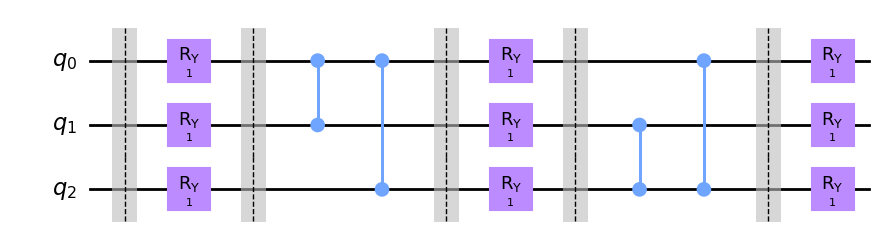
\includegraphics[scale=0.6]{img/ansatz.png}
    \end{center}
\end{frame}

\begin{frame}{\textit{Ansatz} grandinė}
    \begin{center}
        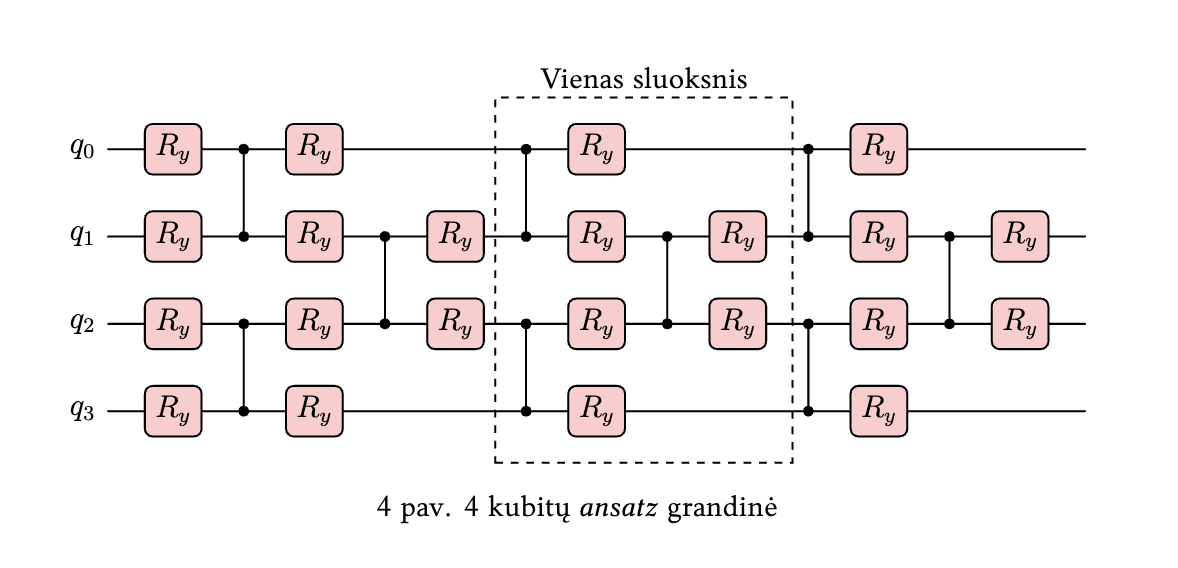
\includegraphics[scale=0.7]{img/ansatz4qubits.png}
    \end{center}
\end{frame}
\begin{frame}{Nuostolių funkcija}
    Sprendžiame performuluotą tiesinių lygčių sistemą:
    $$A |x\rangle \approx |b \rangle \equiv AV(\alpha)|0\rangle \approx |b\rangle$$

    Norint rasti geriausius $\alpha$ reikia minimizuoti nuostolių funkcijos reikšmę \cite{VQLS}:
    \begin{gather}
        H_P \ = \ \mathbb{I} \ - \ |b\rangle \langle b| \nonumber \\ 
        \hat{C}_P \ = \ \frac{\langle \psi | H_P | \psi \rangle \ } {\langle\psi|\psi\rangle} = \frac{\langle \psi | \psi \rangle}{\langle \psi | \psi \rangle} \ - \ \frac{\langle \psi |b\rangle \langle b | \psi \rangle}{\langle \psi | \psi \rangle} \ = \ 1 \ - \ \frac{\langle \psi |b\rangle \langle b | \psi \rangle}{\langle \psi | \psi \rangle} \ = \ 1 \ - \ \frac{|\langle b | \psi \rangle|^2}{\langle \psi | \psi \rangle} \nonumber
     \end{gather}
\end{frame}

\begin{frame}{$\langle \psi|\psi\rangle$ apskaičiavimas}
    \begin{gather}
        \langle \psi | \psi \rangle \ =  \langle 0 | V(\alpha)^{\dagger} A^{\dagger} A V(\alpha) |0\rangle \ = \ \langle 0 | V(\alpha)^{\dagger} \Big( \displaystyle\sum_{m} c_m \ A_m \Big)^{\dagger} \Big( \displaystyle\sum_{n} c_n \ A_n \Big) V(\alpha) |0\rangle = \nonumber \\ 
        = \sum_{m} \sum_{n} \overline{c_{m}} c_{n} \langle 0 | V(\alpha)^\dag A_{m}^\dag A_{n} V(\alpha)|0\rangle \nonumber
    \end{gather}
    \begin{center}
        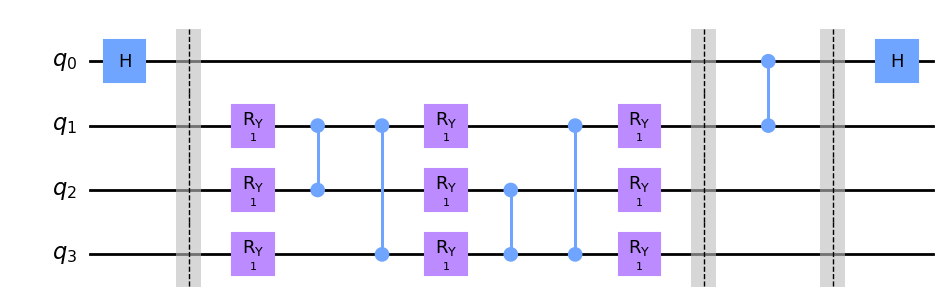
\includegraphics[scale=0.6]{img/hadamardTest.png}
    \end{center}
\end{frame}

\begin{frame}{Taisyklės}
    \begin{center}
        \includegraphics[scale=0.3]{img/rules.png}
    \end{center}
\end{frame}

\begin{frame}{$|\langle b|\psi \rangle|^2$ apskaičiavimas}
    \begin{gather}
         |\langle b | \psi \rangle|^2 \ = \ |\langle b | A V(\alpha) | 0 \rangle|^2 \ = \ |\langle 0 | U^{\dagger} A V(\alpha) | 0 \rangle|^2 \ = \ \langle 0 | U^{\dagger} A V(\alpha) | 0 \rangle \langle 0 | V(\alpha)^{\dagger} A^{\dagger} U |0\rangle = \nonumber \\
        = \ \displaystyle\sum_{m} \displaystyle\sum_{n} \overline{c_m} c_n \langle 0 | U^{\dagger} A_n V(\alpha) | 0 \rangle \langle 0 | V(\alpha)^{\dagger} A_m^{\dagger} U |0\rangle \nonumber
    \end{gather}
     \begin{center}
        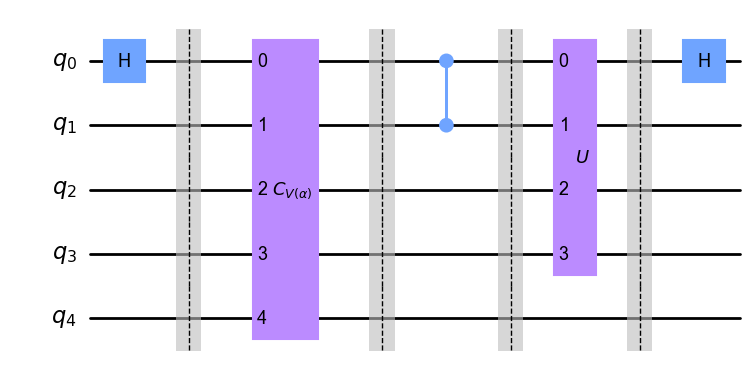
\includegraphics[scale=0.55]{img/specialHadamardTest.png}
    \end{center}
\end{frame}

\begin{frame}{VQLS-SVM algoritmas}
    \begin{center}
        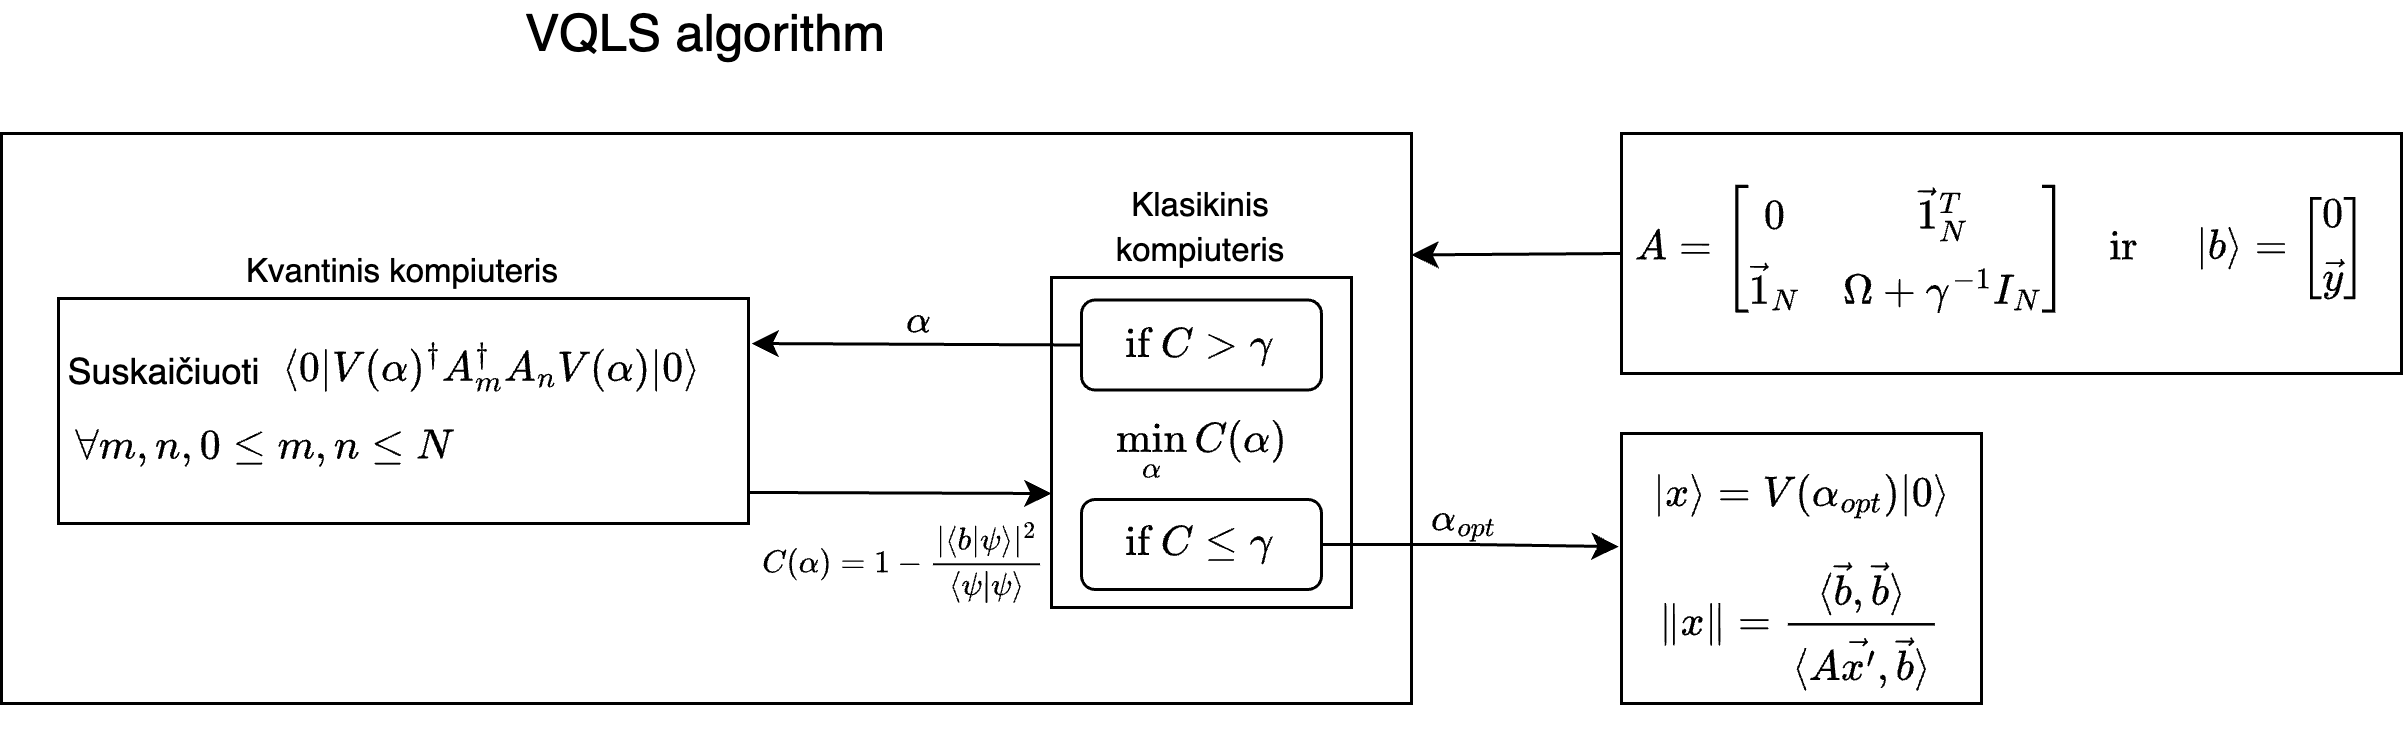
\includegraphics[scale=0.18]{img/VQLS.drawio.png}
    \end{center}
\end{frame}